% !TeX root = ../main.tex
\newcounter{paperalgorithm}
\newenvironment{paperalgorithm}[2]{%
  \par\Needspace{15\baselineskip}\refstepcounter{paperalgorithm}\label{#2}%
  \begingroup\small\setstretch{1.05}\setlength{\parskip}{4pt}%
  \noindent\rule{\linewidth}{0.6pt}\par\noindent\textbf{算法\thepaperalgorithm\quad #1}\par
}{\par\noindent\rule{\linewidth}{0.6pt}\par\endgroup}

\begin{paperalgorithm}{供暖季求解与复核流程}{alg:season-workflow}
\noindent\textbf{输入：}场景配置、规划输入、连续供暖季逐时数据和求解容差。\par
\noindent\textbf{输出：}投资及逐时运行方案，求解状态、间隙和校核记录。
\begin{enumerate}[label=\arabic*.,leftmargin=1.8em,itemsep=2pt,topsep=3pt,parsep=0pt]
\item 核对时间范围、步长、缺测及单位；读取各模块启用状态与参数来源。
\item 装配源、网、荷、储及电力接口；对所有小时联立守恒、容量和热状态约束，设置初始及期末边界。
\item \textbf{若采用联合求解：}在完整声明窗口同时求投资与运行方案。
\item \textbf{若采用固定投资复算：}求得规划方案或读入已登记方案；将全部投资项冻结为存量，保持可靠性条件，再构造全季运行模型并求解。
\item 保存可行解、求解状态、上下界及相对间隙；无可行解时随异常报告失败原因，结束本次计算。
\item 按实际启用模块，复核逐时平衡、容量、储热边界、舒适约束与服务期覆盖；校核不通过则保留记录并标记未通过。
\item 导出配置、投资、逐时运行与检查结果；分别标注联合模型可行解或固定投资下可行解。
\end{enumerate}
\end{paperalgorithm}

\begin{paperalgorithm}{独立费用—碳排放采样接口}{alg:epsilon-workflow}
\noindent\textbf{输入：}同一配置和时间序列、碳帽档数$K\geq2$。\par
\noindent\textbf{输出：}通过复核的采样非支配方案、边际减排费用和折中建议。
\begin{enumerate}[label=\arabic*.,leftmargin=1.8em,itemsep=2pt,topsep=3pt,parsep=0pt]
\item 复制输入配置，清除原碳帽并令碳价为零；保留设备、运行与可靠性约束。
\item 分别以费用和排放为主目标求端点；第二阶段约束主目标不高于第一阶段可行值加容差，再优化次目标。
\item 检查端点排放的先后关系；不满足容差要求则终止，满足时在两端排放值间等距设置$K$档碳帽。
\item \textbf{对每档碳帽：}复制同一基础配置，加数值容差后施加碳帽；按费用目标重新构模并求解。投资项是否固定取决于输入配置。
\item 对本档解独立检查数值残差和碳帽；任一检查不通过则报错并终止扫描，通过则保存全部结果。
\item 对通过的样本去重并剔除受支配点，计算相邻方案的边际减排费用；用归一化理想点距离给出折中建议。
\end{enumerate}
\end{paperalgorithm}

算法\ref{alg:epsilon-workflow}对应当前代码的独立接口，流程见图\ref{fig:epsilon-workflow-a2}。所得集合限于已采样可行解，折中建议取决于归一化规则。供暖季历史扫描保留其原记录中的碳价与偏好，不与这一接口混记。

\begin{figure}[H]
\centering
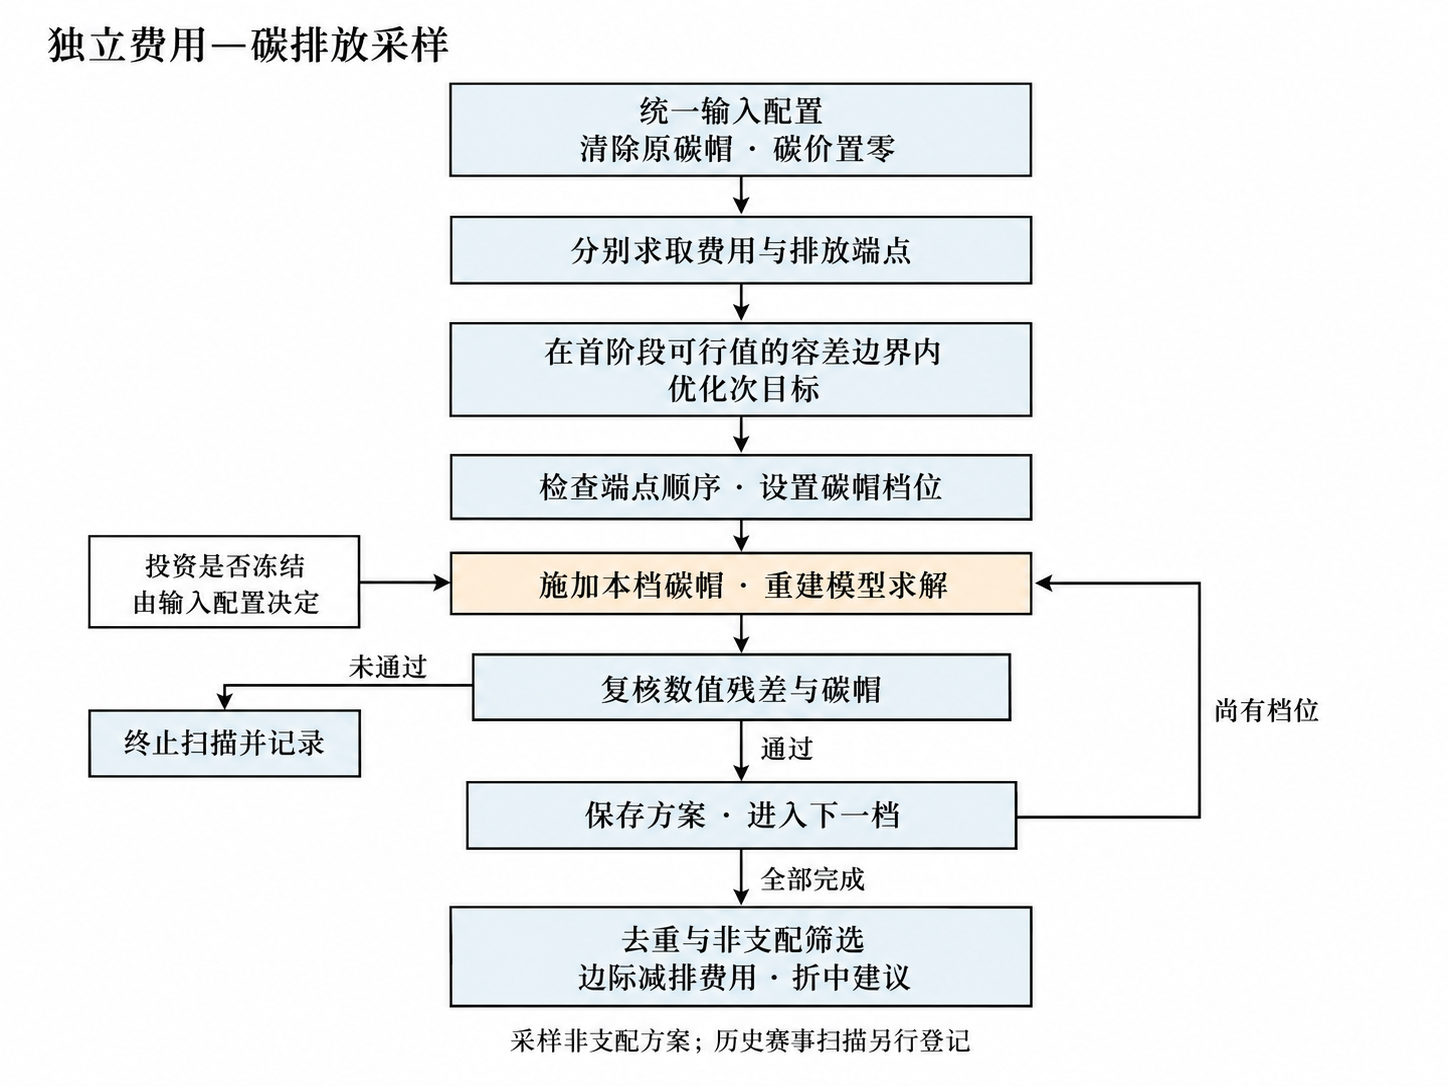
\includegraphics[width=\textwidth]{media/algorithm-revision/epsilon_workflow_a2.png}
\caption{独立费用---碳排放采样与复核流程}
\label{fig:epsilon-workflow-a2}
\end{figure}
